%%%%%%%%%%%%%%%%%%%%%%%%%%%%%%%%%%%%%%%%%
%  Telemac Documentation
%  Git guide
%
%%%%%%%%%%%%%%%%%%%%%%%%%%%%%%%%%%%%%%%%%

%----------------------------------------------------------------------------------------
%	PACKAGES AND OTHER DOCUMENT CONFIGURATIONS
%----------------------------------------------------------------------------------------
\documentclass[Misc]{../../data/TelemacDoc} % Default font size and left-justified equations
%\documentclass[Telemac2D,french]{TelemacDoc} % Default font size and left-justified equations in french
% set font for software
\newcommand{\soft}[1]{{\texttt{\color{blue} #1}}}
\newcommand{\file}[1]{{\texttt{\color{orange} #1}}}
\newcommand{\important}[1]{{\textbf{\color{orange} #1}}}
\newcommand{\crixus}{\soft{Crixus}}
\newcommand{\gmsh}{\soft{Gmsh}}
\newcommand{\blender}{\soft{Blender}}
\newcommand{\paraview}{\soft{Paraview}}
\newcommand{\spartacus}{\soft{Spartacus}}
\newcommand{\sphynx}{\soft{Sphynx}}

%---------------------------------------------------------------------------
% Code format
%---------------------------------------------------------------------------
\usepackage{listings}
\lstset{%language=bash,
	basicstyle=\ttfamily,	% the size of the fonts that are used for the code
	tabsize=4,
%	commentstyle=\color{orange},
%	numbers=left,				% where to put the line-numbers; possible values are (none, left, right)
%	numbersep=5pt,				% how far the line-numbers are from the code
%	numberstyle=\tiny\color{darkgray}	% the style that is used for the line-numbers
}

\begin{document}

\let\cleardoublepage\clearpage

%----------------------------------------------------------------------------------------
%	TITLE PAGE
%----------------------------------------------------------------------------------------
\title{\tel \mbox{\scshape{system}}}
\subtitle{Git Guide}
\version{\telmaversion}
\date{\today}
\maketitle
\clearpage


%----------------------------------------------------------------------------------------
%	COPYRIGHT PAGE
%----------------------------------------------------------------------------------------

\newpage

\thispagestyle{empty}

\TelemacCopyright{}


%----------------------------------------------------------------------------------------
%	TABLE OF CONTENTS
%----------------------------------------------------------------------------------------


\pagestyle{empty} % No headers

\tableofcontents% Print the table of contents itself

%\cleardoublepage % Forces the first chapter to start on an odd page so it's on the right

\pagestyle{fancy} % Print headers again

%==================================
%==================================
\chapter{Introduction}
%==================================
%==================================
%==================================
\section{A word of caution}
%==================================
This document contains information about the quality of a complex modelling tool. Its purpose is to assist the user in assessing the reliability and accuracy of computational results, and to provide guidelines with respect to the applicability and judicious employment of this tool. This document does not, however, provide mathematical proof of the correctness of results for a specific application. The reader is referred to the License Agreement for pertinent legal terms and conditions associated with the use of the software.

The contents of this validation document attest to the fact that computational modelling of complex physical systems requires great care and inherently involves a number of uncertain factors. In order to obtain useful and accurate results for a particular application, the use of high-quality modelling tools is necessary but not sufficient. Ultimately, the quality of the computational results that can be achieved will depend upon the adequacy of available data as well as a suitable choice of model and modelling parameters.
% 
%==================================
\section{Validation layout}
% %==================================

This validation is presented hereafter using a \textit{validation sheet form},
each sheet detailing the physical concepts involved, the physical and numerical parameters used and comparing both numerical and reference solutions.
Then, each sheet displays the following informations:
\begin{list}{-}{}
\item [-] \textbf{Purpose \& Problem description} : These first two parts give reader short details about the test case, the physical phenomena involved and specify how the numerical solution will be validated;
\item [-] \textbf{Reference} : This part gives the reference solution we are comparing to and explicits the analytical solution when available;
\item [-] \textbf{Physical parameters} : This part specifies the geometry,
details all the physical parameters used to describe both porous media (soil model in particularly) and
solute characteristics (dispersion/diffusion coefficients, soil $\equiv$ pollutant interactions...);
\item [-] \textbf{Geometry and Mesh} : This part describes the mesh used in the \tomawac computation;
\item [-] \textbf{Initial and boundary conditions} : this part details both initial and boundary conditions used to simulate the case ;
\item [-] \textbf{Numerical parameters} : this part is used to specify the numerical parameters used
(adaptive time step, mass-lumping when necessary...);
\item [-] \textbf{Results} : we comment in this part the numerical results against the reference ones,
giving understanding keys and making assumptions when necessary.
\end{list}
%
\bigskip
%
\clearpage
%==================================
%==================================
\chapter{Presentation}
%==================================
%==================================
\section{General}
%==================================
\tomawac is a scientific software which models the changes, both in the time and in the spatial domain, of the power spectrum of wind-driven waves and wave agitation for applications in the oceanic domain, in the intracontinental seas as well as in the coastal zone. The model uses the finite elements formalism for discretizing the sea domain; it is based on the computational subroutines of the TELEMAC system as developed by the EDF R\&D’s Laboratoire National d'Hydraulique et Environnement (LNHE). \tomawac is one of the models making up the TELEMAC system 
The acronym \tomawac being adopted for naming the software was derived from the following English denomination:

TELEMAC-based Operational Model Addressing Wave Action Computation

\tomawac can be used for three types of applications:
\begin{itemize}
\item	Wave climate forecasting a few days ahead, from wind field forecasts. This real time type of application is rather directed to weather-forecasting institutes such as Météo-France, whose one mission consists in predicting continuously the weather developments and, as the case may be, publishing storm warnings.
\item	Hindcasting of exceptional events having severely damaged maritime structures and for which field records are either incomplete or unavailable.
\item	Study of wave climatology and maritime or coastal site features, through the application of various, medium or extreme, weather conditions in order to obtain the conditions necessary to carry out projects and studies (harbour constructions, morphodynamic coastal evolutions, ...).
\end{itemize}

%==================================
\section{Capabilities}
%==================================
 \subsection{Application domain of the model \tomawac}
\label{par31}
\tomawac is designed to be applied from the ocean domain up to the coastal zone. The limits of the application range can be determined by the value of the relative depth d/L, wherein d denotes the water height (in metres) and L denotes the wave length (in metres) corresponding to the peak spectral frequency for irregular waves.

The application domain of \tomawac includes:
\begin{itemize}
\item {\bf the oceanic domain}, characterized by large water depths, i.e. by relative water depths of over 0.5. The dominant physical processes are: wind driven waves, whitecapping dissipation and non-linear quadruplet interactions.
\item {\bf the continental seas and the medium depths}, characterized by a relative water depth ranging from 0.05 to 0.5. In addition to the above processes, the bottom friction, the shoaling (wave growth due to a bottom rise) and the effects of refraction due to the bathymetry and/or to the currents are to be taken into account.
\item {\bf The coastal domain}, including shoals or near-shore areas (relative water depth lower than 0.05). For these shallow water areas, such physical processes as bottom friction, bathymetric breaking, non-linear triad interactions between waves should be included. Furthermore, it could be useful to take into account the effects related to unsteady sea level and currents due to the tide and/or to the weather-dependent surges.
\end{itemize}

Through a so-called finite element spatial discretization, one computational grid may include mesh cells among which the ratio of the largest sizes to the smallest ones may reach or even exceed 100. That is why \tomawac can be applied to a sea domain that is featured by highly variable relative water depths; in particular, the coastal areas can be finely represented.

The application domain of \tomawac does not include the harbour areas and, more generally, all those cases in which the effects of reflection on structures and/or diffraction may not be ignored.

A first version of a diffraction model is available in \tomawac and is able to represent some diffraction effects. The model presents still some limits. It is highly recommended to use phase-resolving models when a detailed simulation of diffraction effects is required (e.g. harbor agitation).

\subsection{Wave interactions with other physical factors}
Several factors are involved in the wave physics and interact to various extents with the waves changing their characteristics. The following main factors should be mentioned:
\begin{itemize}
\item bathymetry and sea bottom geometry (bottom friction, refraction, surf-breaking, non-linear effects of interactions with the bottom, sand rippling...)
\item atmospheric circulation (wind and pressure effects)
\item tide pattern (variation of currents and water heights),
\item three-dimensional oceanic circulation currents,
\item over/underelevations caused by exceptional weather events, resulting in sea levels variations up to several meters (storm, surges).
\end{itemize}
The fine modelling of the interactions between these various physical factors and the waves is generally rather complex and several research projects are currently focused on it. Within the application domain as defined in the previous paragraph, \tomawac models the following interactions:
\begin{itemize}

\item {\bf wave-bathymetry interaction}: the submarine relief data input into \tomawac are constant in time, but the sea level can change in time. In addition to the effects of the sea level variations in time, \tomawac allows to take into account refraction, shoaling, bottom friction and bathymetric breaking. \tomawac simulations can take into account some diffraction effects.
\item {\bf wave-atmosphere interaction}: this interaction is the driving phenomenon in the wave generation, takes part in energy dissipation processes (whitecapping, wave propagation against the wind…) and is involved in the energy transfer. To represent the unsteady behaviour of this interaction, \tomawac requires 10 m wind fields (specification of the couple of horizontal velocity components) with a time step matched to the weather conditions being modelled. These wind fields can be provided either by a meteorological model or from satellite measurements.
\item {\bf wave-current interaction}: the sea currents (as generated either by the tide or by oceanic circulations) may significantly affect the waves according to their intensity. They modify the refractive wave propagation direction, they reduce or increase the wave height according to their propagation direction in relation to the waves and may influence the wave periods if exhibiting a marked unsteady behaviour. In \tomawac, the current field is provided by the couple of horizontal components of its average (or depth-integrated) velocity at the nodes of the computational grid. \tomawac allows to model the frequency changes caused either by the Doppler effect or by the unsteady currents, as well as by an heterogeneous current field.
\end{itemize}
\subsection{ The physical processes modelled in \tomawac}
Those interactions being taken into account by \tomawac have been reviewed and a number of physical events or processes have been mentioned in the previous paragraph. These processes modify the total wave energy as well as the directional spectrum distribution of that energy (i.e. the shape of the directional spectrum of energy). So far, the numerical modelling of these various processes, although some of them are now very well known, is not yet mature and keep on providing many investigation subjects. Considering the brief review of physical interactions given in the previous paragraph, the following physical processes are taken into account and digitally modelled in \tomawac:

{\bf—> Energy source/dissipation processes:}
\begin{itemize}
\item wind driven interactions with atmosphere. Those interactions imply the modelling of the wind energy input into the waves. It is the prevailing source term for the wave energy directional spectrum. The way that spectrum evolves primarily depends on wind velocity, direction, time of action and fetch (distance over which the wind is active). It must be pointed out that the energy which is dissipated when the wind attenuates the waves is not taken into account in \tomawac.
\item 	whitecapping dissipation or wave breaking, due to an excessive wave steepness during wave generation and propagation.
\item 	bottom friction-induced dissipation, mainly occurring in shallow water (bottom grain size distribution, ripples, percolation...)
\item 	dissipation through bathymetric breaking. As the waves come near the coast, they swell due to shoaling until they break when they become to steep.
\item dissipation through wave blocking due to strong opposing currents.
\end{itemize}
{\bf—> Non-linear energy transfer conservative processes:}
\begin{itemize}
\item 	non-linear resonant quadruplet interactions, which is the exchange process prevailing at great depths.
\item 		non-linear triad interactions, which become the prevailing process at small depths.
\end{itemize}
{\bf—> Wave propagation-related processes:}
\begin{itemize}
\item 	 wave propagation due to the wave group velocity and, in case, to the velocity of the medium in which it propagates (sea currents).
\item 	depth-induced refraction which, at small depths, modifies the directions of the wave-ray and then implies an energy transfer over the propagation directions.
\item 	shoaling: wave height variation process as the water depth decreases, due to the reduced wavelength and variation of energy propagation velocity.
\item 	current-induced refraction which also causes a deviation of the wave-ray and an energy transfer over the propagation directions.
\item 	interactions with unsteady currents, inducing frequency transfers (e.g. as regards tidal seas).
\item 	diffraction by a coastal structure (breakwater, pier, etc…) or a shoal, resulting in an energy transfer towards the shadow areas beyond the obstacles blocking the wave propagation. The current version of the diffraction model implemented in \tomawac is able to represent qualitatively some diffraction effects.
\end{itemize}

It should be remembered that, due to the hypothesis adopted in paragraph \ref{par31} about the \tomawac application domain, the reflection (partial or total) from a structure or a pronounced depth irregularity is not addressed by the model.



\chapter{Using \soft{Git} for TELEMAC-MASCARET}

In this chapter, we will see how to start using \soft{Git} for development with
TELEMAC-MASCARET.

\section{Cloning the repository}

The TELEMAC-MASCARET source code is currently hosted on a GitLab server
maintained by EDF R\&D and available at
\url{https://gitlab.pam-retd.fr/otm/telemac-mascaret}. 

You have to \important{clone} this \soft{Git} repository, and by default the
entire repository is cloned. Options to limit the size of the cloned repository
on your local system are available and provided below.

\subsection{Complete clone}
From a terminal:
\begin{small}
\begin{lstlisting}
$ git clone https://gitlab.pam-retd.fr/otm/telemac-mascaret.git
  my_opentelemac
$ cd my_opentelemac
\end{lstlisting}
\end{small}

Here the clone will be made within the directory named
\important{my\_opentelemac} but you can name it as you wish.

\subsection{Single branch clone}
It is possible to clone a single branch as follows:
\begin{small}
\begin{lstlisting}
$ git clone -b feature_branch --single-branch
  https://gitlab.pam-retd.fr/otm/telemac-mascaret.git
  my_opentelemac/feature_branch
\end{lstlisting}
\end{small}

The disadvantage of this process is that you can no longer recover another
branch within \important{my\_opentelemac} without doing a low-level
manipulation on the local repository. Therefore, cloning a single branch is not
recommended, unless you work in a separate directory for each branch.

\subsection{Shallow clone}
It is also possible to make a “shallow clone” which consists in limiting the
history to a certain number of commits. For example, to retrieve the last 20
commits only:

\begin{small}
\begin{lstlisting}
$ git clone --depth 20
  https://gitlab.pam-retd.fr/otm/telemac-mascaret.git
\end{lstlisting}
\end{small}

However, this method is not recommended either outside of a repository
submodule or a continuous integration environment.

\subsection{Partial clone}
Finally, it is possible to make a “partial clone” by filtering the directories,
which consists in recovering only part of the \soft{Git} repository. This
process requires a recent version of \soft{Git} as well as the presence of a
filter file on the system repository.\\
\\
For TELEMAC-MASCARET, such file has been included on the repository that
ignores the examples. Other filter files can be added upon request. The
\soft{Git} command is as follows:
\begin{small}
\begin{lstlisting}
$ git clone --sparse --filter=sparse:oid=main:.gitfilterspec
  https://gitlab.pam-retd.fr/otm/telemac-mascaret.git my_opentelemac
$ cd my_opentelemac
$ git config --local core.sparsecheckout true
$ git show origin/main:.gitfilterspec >> .git/info/sparse-checkout
$ git checkout main
\end{lstlisting}
\end{small}

The above list of commands is quite heavy as \soft{Git} is not at all intended
for partial clone, but it works.

\section{Cloning the repository -- GUI users}
All GUI clients provide a clone command located under the main menu, for
example in ``Repository > Clone'' for \soft{SmartGit}, or
``Start > Clone Repository…'' for \soft{Git Extensions}.\\
\\
Most interfaces provide you with direct access to single branch and/or shallow
clone. You can do a partial clone using the command line description above.

\section{Configuring developer credentials}
People who requested a developer access should all have received an e-mail to
access the GitLab server when their account was created.\\

If the identifiers are not necessary to clone the repository, since it is
public, it is obviously not the same to modify it. Access rights are required
through a two-factor authentication (2FA). Both authentication factors are
required every time you log on to GitLab.\\

The first level authentication factor is your GitLab username and password. The
second level factor is a code that is generated through an OTP (One-Time
Password) application that you have to install on another device, such as your
phone. Such applications include FreeOTP or Microsoft Authenticator, but many
others are available for Android and iOS.\\

Fortunately, this OTP is only necessary when accessing the GitLab web page. But
when working with \soft{Git}, the access is stored locally on your system in
the form of a personal \important{access token}.\\

To generate this token, you need first to connect to the GitLab web interface.
On that occasion, you will need your GitLab username and password as well as
the OTP code. Once logged on, the access token is available through
\important{Edit profile}, selecting \important{Access Tokens}.\\

You must then generate the access token by filling in a name (of the
application that uses \soft{Git}, for instance) and making sure that you have
checked \important{read\_repository} and \important{write\_repository} at
least.\\

Then click on \important{Create personal access token} for the key to appear at
the top of the page: note it down, copy/paste it, keep it, as you will lose it
once you leave the web page.

\subsection{Linux users}
In order to avoid entering the token each time you push to the repository, you
need to enter the following command to store your credentials:
\begin{small}
\begin{lstlisting}
$ git config --global credential.helper store
\end{lstlisting}
\end{small}

Then, the token is to be written to \$HOME/.git-credentials in the following
form:\\
\url{https://oauth2:<TOKEN>@gitlab.pam-retd.fr}\\
Of course, you will need to replace \important{<TOKEN>} with your own token.\\

From here you can work.

\subsection{Windows users}
Since \soft{Git} \important{Credential Manager Core} should have been enabled
through the \soft{Git} setup, storing your credentials requires only to enter
the token once and for all, for example when cloning the repository (or later
on, when doing a push):

\begin{small}
\begin{lstlisting}
$ git clone
  https://oauth2:<TOKEN>@gitlab.pam-retd.fr/otm/telemac-mascaret.git
  my_opentelemac
\end{lstlisting}
\end{small}

\section{Configuring the repository}
Before to start working with \soft{Git}, you need to indicate the username
and e-mail address that will be associated with the commits.\\

For TELEMAC-MASCARET, we recommend using your first and last name, by entering,
from the repository directory:
\begin{small}
\begin{lstlisting}
$ git config user.name "FirstName LastName"
$ git config user.email firstname.lastname@mycompany.com
\end{lstlisting}
\end{small}

You can also configure \soft{Git} to use the text editor of your choice for
editing commit messages. Otherwise, the default \soft{Git} interface will be
used. To set it (.e.g to use \soft{Emacs}), enter:
\begin{small}
\begin{lstlisting}
$ git config core.editor emacs
\end{lstlisting}
\end{small}

To use the same settings for all your \soft{Git} repositories, you need to pass
the \important{global} option to the above commands, e.g.:
\begin{small}
\begin{lstlisting}
$ git config --global core.editor emacs
\end{lstlisting}
\end{small}

\subsection{Proxy settings}

If your organization is behind a proxy you need to tell Git to use it as below:
\begin{small}
\begin{lstlisting}
$ git config --global
  http.proxyhttps://<username>:<password>@<proxy_address>:<proxy_port>
$ git config --global
  https.proxy https://<username>:<password>@<proxy_address>:<proxy_port>
\end{lstlisting}
\end{small}

By replacing:
\begin{itemize}
  \item <proxy\_address>: by the address to your proxy;
  \item <proxy\_port>: by the port of your proxy;
  \item <username>: by the login to your proxy, if any;
  \item <password>: by the password to your proxy, if any.
\end{itemize}

\chapter{Working on branches with \soft{Git}}\label{sec:useGit}

\section{Creating a branch}
\soft{Git} saves snapshots of your project when you make commits, and
\important{always} attributes them to the \important{branch} on which you are
located. A branch is composed by a ``homogeneous'' set of commits: for example,
you can have a branch containing all your stable version project, a branch
containing the future stable version, development branches where you introduce
a new feature in the code, etc.\\

The branch \important{main} is created by default. We usually use it for stable
versions of the code.\\

To add a new branch, enter:
\begin{lstlisting}
$ git branch my_branch
\end{lstlisting}
To remove a branch, enter:
\begin{lstlisting}
$ git branch -d my_branch
\end{lstlisting}

To tell \soft{Git} you want to work on a specific branch, enter:
\begin{lstlisting}
$ git checkout my_branch
\end{lstlisting}
Then all the subsequent commits will be done in \important{my\_branch}.

\section{Developing on branches}

Once you have told \soft{Git} to position you on a branch, you can start to
work on it by modifying the existing files or by adding new ones.\\

\important{Important}: before committing, you need to specify which files will
be committed by adding them to the \important{stage area}. Files which are not
added to this space will not be part of the next commit.\\

Therefore, to include a modified or created file in the next commit, you need
to enter:
\begin{lstlisting}
$ git add filename.ext
\end{lstlisting}
You can also choose to only add part of the modifications that you have made to
a file, using the \important{-p} option:
\begin{lstlisting}
$ git add -p filename.ext
\end{lstlisting}
Then \soft{Git} asks you directly from the terminal if you want to stage
($\equiv$ to add) each part of your modifications (\soft{Git} identifies them
as blocks of modifications). For each part that you want to add, type
\important{y} and enter, otherwise \important{n} and enter.\\

To remove a file versioned from the repository, you need to enter:
\begin{lstlisting}
$ git rm filename.ext
\end{lstlisting}

To remove files from the \important{stage area}, e.g. if you added a file by
mistake, enter:
\begin{lstlisting}
$ git reset -- filename.ext
\end{lstlisting}

Once you have added and/or removed all the files you wanted, you can commit
them:
\begin{lstlisting}
$ git commit -m "My commit message"
\end{lstlisting}

\important{The commit message should describe the changes and should not exceed
72 characters.}\\

You can also enter a more detailed message by using the text editor. To do so,
do not specify a message when calling the \important{commit} command, as below:
\begin{lstlisting}
$ git commit
\end{lstlisting}
\soft{Git} then pops up a text editor window and asks you to enter a
\important{commit message}. Enter the message, then save and close the
editor.\\

After a commit, \soft{Git} tells you a new commit has been made on the branch:
\begin{footnotesize}
\begin{lstlisting}
[main 537e9e633] My commit message
1 file changed, 0 insertions(+), 0 deletions(-)
create mode 100644 sources/telemac2d/my_new_file.f
\end{lstlisting}
\end{footnotesize}

\important{Note}: you can choose to commit all the modifications that have been
made in the currently tracked files by doing as follows:
\begin{lstlisting}
git commit -a "My commit message"
\end{lstlisting}
However, this command will not include new files.

\subsection{Commit messages}
Commit messages are quite important so here are some tips to make them better:
\url{http://robots.thoughtbot.com/5-useful-tips-for-a-better-commit-message}\\

You should structure your commit message like this (from 
\url{http://git-scm.com/book/ch5-2.html}):
\begin{footnotesize}
\begin{lstlisting}
Short (50 chars or less) summary of changes

More detailed explanatory text, if necessary.  Wrap it to about 72
characters or so. In some contexts, the first line is treated as the
subject of an email and the rest of the text as the body.  The blank
line separating the summary from the body is critical (unless you omit
the body entirely); tools like rebase can get confused if you run the
two together.

Further paragraphs come after blank lines.

 \- Bullet points are okay, too

 \- Typically a hyphen or asterisk is used for the bullet, preceded by a
   single space, with blank lines in between, but conventions vary here
\end{lstlisting}
\end{footnotesize}

\subsection{Best practices}
Commit your developments very regularly.\\

For each sub-development, a commit should be done: when you create a new
function, a new variable, a new class, when you fix a bug, etc.\\

Do not hesitate to do a lot of commits: once your development are finished,
you can squash them to fewer and larger commits for better readability of the
commit history (see below).\\

A commit may only contain modifications of a few lines in one file as long as
that modification has a significant impact.\\

One useful thing is that you can navigate in the branch to find out where a bug
was introduced (making a dichotomy is usually fast). Therefore, it is important
that \important{for every commit you make, the code has to compile without
errors}. Otherwise, bug tracking is made very difficult.

\section{Useful commands}

The command:
\begin{lstlisting}
$ git log
\end{lstlisting}
shows the history of your branches, where you can see that an ID was assigned
to each commit. This ID is SHA-1 hash of every important thing about the
commit. You can also get commit IDs from your GUI client, such as
\soft{gitk}.\\

You can revert the modifications introduced in a commit by entering:
\begin{lstlisting}
$ git revert commit_id
\end{lstlisting}

You can see the differences in a file between the current and a previous
version by entering:
\begin{lstlisting}
git difftool commit_id filename.ext
\end{lstlisting}
where the diff tool may be \soft{vimdiff} or \soft{meld}, for instance.\\

To set the tool used by git type:
\begin{lstlisting}
git config diff.tool meld
\end{lstlisting}

\section{Move inside or in between branches}

You can always come back to any version of your project by coming back to the
corresponding commit.\\

To move to a given branch:
\begin{lstlisting}
$ git checkout branch_name
\end{lstlisting}

To position the repository at a given commit:
\begin{lstlisting}
$ git checkout commit_id
\end{lstlisting}

\soft{Git} will usually refuse to move if you have uncommitted changes in your
project. To see the uncommitted changes, enter:
\begin{lstlisting}
$ git status
\end{lstlisting}

If you want to \important{move and erase the uncommitted changes} (which may be
quite risky):
\begin{lstlisting}
$ git checkout -f commit_id
\end{lstlisting}

If you want to temporarily save your changes to be able to recover them later:
\begin{lstlisting}
$ git stash
\end{lstlisting}

The stash is a space for saving temporary changes that you may want to apply
later.\\

You may now move around in the history unhindered. You may have several sets of
modifications in the stash, you can list them by entering:
\begin{lstlisting}
$ git stash list
\end{lstlisting}
Each stash has a number assigned to it (stash$\{0\}$, stash$\{1\}$, etc.).\\

Apply the changes contained in one of the stashes (here the number 3):
\begin{lstlisting}
$ git stash apply stash{3}
\end{lstlisting}
Entering only \important{git stash apply} will apply the changes contained in
stash$\{0\}$.\\

Erase the content of given stash (here number 3):
\begin{lstlisting}
$ git stash drop stash{3}
\end{lstlisting}
Entering only \important{git stash drop} will drop the changes contained in
stash$\{0\}$.\\

Apply and erase the changes contained in one of the stashes (here number 3):
\begin{lstlisting}
$ git stash pop stash{3}
\end{lstlisting}
Entering only \important{git stash pop} will apply and erase the changes
contained in stash$\{0\}$.

\section{Merge developments in between branches}

A very interesting feature of \soft{Git} is that it allows you to apply the
changes made in one branch to another one quite easily. There are two commands
for this, namely \important{git merge} and \important{git rebase}. Here we will
focus on rebasing. The two techniques are quite equivalent, but rebasing is
considered cleaner and as such, is used as a coding convention in
TELEMAC-MASCARET.\\

Let's say you have created a branch called \important{my\_branch} that you have
used to develop a new feature. In the meanwhile, someone has made developments
in the branch \important{other\_branch}, and you now want to apply your
development to \important{other\_branch}.\\

First, if \important{other\_branch} is a shared branch, you may not want to
share all the commits you have done with such a degree of detail as for your
personal use.
Therefore, it is recommended to follow the process below:
\begin{itemize}
\item Backup your branch:
\begin{lstlisting}
$ git branch my_branch_backup
\end{lstlisting}

\item Modify the commit history by using an interactive rebase:
\begin{lstlisting}
$ git rebase -i HEAD~5
\end{lstlisting}
This command will prompt the text editor where the 5 latest commits (any number
works of course) in the branch are displayed. You can then decide to squash
some of them (put them together), reword the commit messages, edit the content
of the commits.\\

The way you can do it is explained in the text file that \soft{Git} prompted
for the interactive rebase. If you change the position of the commit in the
column, it will modify the order of the commit in the branch accordingly.
Deleting a commit in the text editor also deletes it in your branch.\\

Note that giving a commit ID for the interactive rebase also works:
\begin{lstlisting}
$ git rebase -i commit_id
\end{lstlisting}

\item Once you have cleaned the branch as you wish, rebase it on top of
\important{other\_branch}:
\begin{lstlisting}
$ git rebase other_branch
\end{lstlisting}
This will move the branch \important{my\_branch} on top of
\important{other\_branch}.\\

In case the same file was modified at the same place in the two branches,
\soft{Git} won't be able to automatically do the rebase and will notify a
conflict in the file. It will stop the rebase and edit the conflictual files,
leaving both versions unmodified to let you choose what you want to keep.
Open the files in a text editor and modify them to remove all the conflicts.
\important{Check that the code correctly compiles after your modifications.}\\

After the files have been edited, you need to add them:
\begin{lstlisting}
$ git add conflictual_file_1 conflictual_file_2 ...
\end{lstlisting}

Then you can continue the rebase:
\begin{lstlisting}
$ git rebase --continue
\end{lstlisting}

In case you don't want to carry on with the rebase, enter:
\begin{lstlisting}
$ git rebase --abort
\end{lstlisting}

\item Once the rebase is done, and you have checked that everything works as
expected (compilation, test-cases), update \important{other\_branch} and remove
\important{my\_branch}:
\begin{lstlisting}
$ git checkout other_branch
$ git merge my_branch
$ git branch -d my_branch
\end{lstlisting}

\end{itemize}


\chapter{TELEMAC-MASCARET \soft{Git} workflow}

In conclusion of this document, the TELEMAC-MASCARET \soft{Git} development
workflow is presented.

\begin{itemize}

\item First make sure all your shared branches are up-to-date with origin:
\begin{lstlisting}
$ git pull --rebase
\end{lstlisting}

\item Create a new local branch and start working on it (make one branch for
each new feature you plan to introduce in the code):
\begin{lstlisting}
$ git checkout -b my_branch
\end{lstlisting}

\item Push your branch to the server:
\begin{lstlisting}
$ git push --set-upstream origin my_branch
\end{lstlisting}

\item Often commit, making small commits containing specific change at a time:
\begin{lstlisting}
$ git add modified_file_1.ext folder/modified_file_2.ext
$ git commit -m "My commit message"
\end{lstlisting}
\important{Note}: use \important{git add -p} if necessary.\\

\important{Before committing, ensure that you have documented all your
changes and that you respect TELEMAC-MASCARET coding conventions.}\\

\important{All the commits must compile for debugging purposes.}

\item Once your developments are finished, you need to merge your branch with
\important{main}. First, backup your branch:
\begin{lstlisting}
$ git branch my_branch_backup
\end{lstlisting}

\item Clean up your branch using an interactive rebase on the necessary amount
of commits (\textit{e.g.} 10):
\begin{lstlisting}
$ git rebase -i HEAD~10
\end{lstlisting}
Follow the text editor instructions to clean your branch history as needed. The
idea is that \important{the history should be kept as clean as possible, so
that it is easily understood by other developers}.

\item Once you have finished cleaning the branch history, create a Merge
Request (MR) by entering the following URL on your web browser:\\
\begin{small}
\url{https://gitlab.pam-retd.fr/otm/test-telemac/-/merge_requests/new?merge_request%5Bsource_branch%5D=my_branch}
\end{small}\\
From the web page, enter a title, describe precisely what your branch does and
create the MR, as in fig.~\ref{fig:mr-creation}.

\begin{figure}[H]
  \centering
  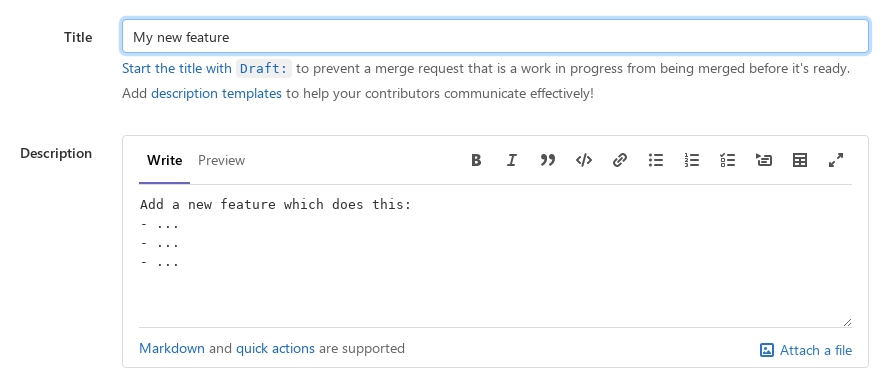
\includegraphics[scale=0.4]{graphics/mr_creation.png}
  \caption{Creation of a Merge Request}
  \label{fig:mr-creation}
\end{figure}

\item If your branch cannot be merged, \soft{GitLab} will disable the
\important{Merge} button and tell you that there are conflicts, as shown in
fig.~\ref{fig:mr-conflicts}.

\begin{figure}[H]
  \centering
  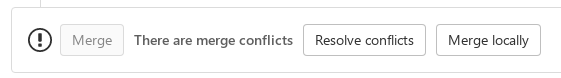
\includegraphics[scale=0.4]{graphics/mr_conflicts.png}
  \caption{Conflicts in a Merge Request}
  \label{fig:mr-conflicts}
\end{figure}

To fix those conflicts, rebase \important{my\_branch} on top of
\important{main}:
\begin{lstlisting}
$ git rebase main
\end{lstlisting}

\item Solve each conflict \soft{Git} encountered during the rebase and
\important{make sure that the code compiles before continuing the rebase}.

\item Once the rebase is finished and that \important{you have verified that
the test-cases run correctly}, force push your branch to update your
\important{MR}:
\begin{lstlisting}
$ git push --force-with-lease
\end{lstlisting}

\important{Important}: you should never use the \important{\texttt{-{}-}force/-f} option
as other developers may have pushed new commits to the branch while you were
rebasing it. Using \important{\texttt{-{}-}force-with-lease} will prevent the update of
a branch in such a case.

\item After conflicts have been solved or if there wasn't any, the
\important{MR} can be accepted. If you have \important{Maintainer} rights on
\soft{GitLab}, you can merge it yourself. However, if the changes brought by
the \important{MR} are quite important, you should ask another developer to
review your changes, a task which can be done from the \important{MR} itself.\\

If you don't have \important{Maintainer} rights, you will need to ask for a
\important{Maintainer} to review your code changes. Maintainers can be found
from the \important{Project members} list which is available from the GitLab
project webpage.\\

\item After the \important{MR} has been accepted, delete your branch if needed
and also delete your backup branch:
\begin{lstlisting}
$ git branch -d my_branch
$ git push origin --delete my_branch
$ git branch -d my_branch_backup
\end{lstlisting}
\end{itemize}

\end{document}
